%%%%%%%%%%%%%%%%%%%%%%%%%%%%%%%%%%%%%%%%%
% Jacobs Portrait Poster
% LaTeX Template
% Version 1.0 (31/08/2015)
% (Based on Version 1.0 (29/03/13) of the landscape template
%
% Created by:
% Computational Physics and Biophysics Group, Jacobs University
% https://teamwork.jacobs-university.de:8443/confluence/display/CoPandBiG/LaTeX+Poster
% 
% Further modified by:
% Nathaniel Johnston (nathaniel@njohnston.ca)
%
% Portrait version by:
% John Hammersley
%
% The landscape version of this template was downloaded from:
% http://www.LaTeXTemplates.com
%
% License:
% CC BY-NC-SA 3.0 (http://creativecommons.org/licenses/by-nc-sa/3.0/)
%
%%%%%%%%%%%%%%%%%%%%%%%%%%%%%%%%%%%%%%%%%

%-------------------------------------------------------------------------------
%	PACKAGES AND OTHER DOCUMENT CONFIGURATIONS
%-------------------------------------------------------------------------------

\documentclass[final]{beamer}

\usepackage[scale=0.8]{beamerposter} % Use the beamerposter package for laying out the poster

\usetheme{confposter} % Use the confposter theme supplied with this template

\setbeamercolor{block title}{fg=ngreen,bg=white} % Colors of the block titles
\setbeamercolor{block body}{fg=black,bg=white} % Colors of the body of blocks
\setbeamercolor{block alerted title}{fg=white,bg=dblue!70} % Colors of the highlighted block titles
\setbeamercolor{block alerted body}{fg=black,bg=dblue!10} % Colors of the body of highlighted blocks
% Many more colors are available for use in beamerthemeconfposter.sty

%-----------------------------------------------------------
% Define the column widths and overall poster size
% To set effective sepwid, onecolwid and twocolwid values, first choose how many columns you want and how much separation you want between columns
% In this template, the separation width chosen is 0.024 of the paper width and a 4-column layout
% onecolwid should therefore be (1-(# of columns+1)*sepwid)/# of columns e.g. (1-(4+1)*0.024)/4 = 0.22
% Set twocolwid to be (2*onecolwid)+sepwid = 0.464
% Set threecolwid to be (3*onecolwid)+2*sepwid = 0.708

\newlength{\sepwid}
\newlength{\onecolwid}
\newlength{\twocolwid}
\newlength{\threecolwid}
\setlength{\paperwidth}{36in} % A0 width: 46.8in
\setlength{\paperheight}{48in} % A0 height: 33.1in
\setlength{\sepwid}{0.024\paperwidth} % Separation width (white space) between columns
\setlength{\onecolwid}{0.22\paperwidth} % Width of one column
\setlength{\twocolwid}{0.464\paperwidth} % Width of two columns
\setlength{\threecolwid}{0.708\paperwidth} % Width of three columns
\setlength{\topmargin}{-0.5in} % Reduce the top margin size
%-----------------------------------------------------------

\usepackage{graphicx}  % Required for including images

\usepackage{booktabs} % Top and bottom rules for tables

\usepackage{url} % Top and bottom rules for tables
\usepackage{fontawesome}
\usepackage[labelformat=empty]{caption}

% Decorate links:
\definecolor{linkcolor}{HTML}{003399}  % from https://gigaom.com/2009/07/09/when-it-comes-to-links-color-matters/
\newcommand{\colorify}[1]{\textcolor{linkcolor}{#1}}
\newcommand{\mylink}[1]{\href{#1}{\colorify{#1}}}
\newcommand{\mylinkn}[2]{\href{#1}{\colorify{#2}}}
\newcommand{\mylinkb}[2]{\href{#1}{#2}}
\newcommand{\mylinkm}[1]{\href{mailto:#1?subject=Your poster at the "Automation in Beamline Control and Data Acquisition" workshop}{\colorify{#1}}}
\newcommand{\mylinkt}[1]{\href{tel:#1}{#1}}

%-------------------------------------------------------------------------------
%	TITLE SECTION 
%-------------------------------------------------------------------------------

\title{\textit{Sirepo}: an open-source cloud-based software interface for X-ray
source and optics simulations} % Poster title


\author{M. S. Rakitin,\inst{a}* P. Moeller,\inst{b, c} R. Nagler,\inst{b} B. Nash,\inst{b} D. L. Bruhwiler,\inst{b} D. Smalyuk,\inst{d} M. Zhernenkov\inst{b} and O. Chubar\inst{b}}
\institute{\faInstitution{}~\inst{a} NSLS-II, Brookhaven National Laboratory, Upton, NY~~~\faInstitution{}~\inst{b} RadiaSoft LLC, Boulder, CO~~~
\faInstitution{}~\inst{c} Bivio Software, Inc., Boulder,~CO~~~\faInstitution{}~\inst{d} Earl L. Vandermeulen High School, Port Jefferson, NY}

%-------------------------------------------------------------------------------

\begin{document}

\addtobeamertemplate{headline}{} 
{
\begin{tikzpicture}[remember picture,overlay] 
\node [shift={(+3.8cm, -4.0cm)}] at (current page.north west){\includegraphics[height=5cm]{images/Sirepo_logo_symbol.png}}; 
\end{tikzpicture} 
}

\addtobeamertemplate{headline}{} 
{
\begin{tikzpicture}[remember picture,overlay] 
\node [shift={(7.0cm, +2.5cm)}] at (current page.south west){
\includegraphics[height=4.0cm]{images/bnl_logo.png}}; 
\end{tikzpicture} 

\begin{tikzpicture}[remember picture,overlay] 
\node [shift={(-8cm, +2.0cm)}] at (current page.south east){
\includegraphics[height=2.5cm]{images/radiasoft_logo.png}}; 
\end{tikzpicture} 
}

\addtobeamertemplate{block end}{}{\vspace*{2ex}} % White space under blocks
\addtobeamertemplate{block alerted end}{}{\vspace*{2ex}} % White space under highlighted (alert) blocks

\setlength{\belowcaptionskip}{2ex} % White space under figures
\setlength\belowdisplayshortskip{2ex} % White space under equations

\begin{frame}[t] % The whole poster is enclosed in one beamer frame

\begin{columns}[t] % The whole poster consists of three major columns, the second of which is split into two columns twice - the [t] option aligns each column's content to the top



%-------------------------------------------------------------------------------
% Left single column
%-------------------------------------------------------------------------------

\begin{column}{\sepwid}\end{column} % Empty spacer column
\begin{column}{\onecolwid} % The first column

\begin{block}{\faInfoCircle{} Abstract}

\textbf{Sirepo} --- an open source cloud-computing framework, which includes a
sophisticated browser-based GUI for X-ray source and optics simulations
\cite{Rakitin2018_Sirepo}. Currently, Sirepo is interfaced with popular codes in
the fields of synchrotron radiation source and optics simulations, such as SRW
and SHADOW3, particle accelerators (Elegant, Hellweg and Warp), and a few
others. Sirepo is a flexible framework that can be relatively easily integrated
with scientific codes to provide a convenient GUI for simulations in the cloud.
\newline \\
\textbf{SRW} (Synchrotron Radiation Workshop) is a physical optics computer
code, allowing simulation of entire experimental beamlines using the concept of
a `virtual beamline' with accurate treatment of synchrotron radiation generation
and propagation through the X-ray optical system \cite{Chubar1998_SRW,
Chubar2002_SRW, Chubar2013_SRW}. SRW is interfaced with Sirepo by means of a
Python API.
\newline \\
Sirepo utilizes interactive widgets and dynamically accessed data from community
databases for X-ray optics \cite{henke, stepanov}. These computational tools are
extensively used for the development and commissioning of new X-ray beamlines
and for testing feasibility and optimization of experiments.
\newline \\

\begin{alertblock}{\faMagic{} Features}
\begin{itemize}

\item \textbf{Sirepo} for SRW contains a number of predefined textbook examples
as well as simulations of the wavefront propagation through existing beamlines
at NSLS-II and LCLS.

\item \textbf{Source} simulation page allows users can simulate and
optimize the source of the synchrotron radiation (e.g. undulator, dipole, etc.)
Contains predefined electron beam and undulator parameters.

\item \textbf{Beamline} simulation page allows to construct a `virtual'
beamline emulating the layout of real X-ray or general optical beamlines. Fully-
and partially-coherent simulations of wavefront propagation can be performed.

\item \textbf{Sirepo} supports most of the optical elements currently used at
beamlines, including recent developments in SRW. Basic simulation of samples is
available via a generic transmission object.

\item Rich interactive visualization and reporting capabilities available in
Sirepo.

\item Publicly available community databases (CXRO, X-ray server) can be
dynamically queried for error-free access to material characteristics.

\item \textbf{Sirepo} works on a local computer, a remote server or a
high-performance cluster. Sirepo is available online and also within the NSLS-II
firewall.

\end{itemize}
\end{alertblock}

\end{block}


\vspace{-0.5cm}
\begin{block}{\faServer{} Server-side implementation}
\vspace{-0.5cm}

\begin{itemize}
  \item \textbf{Python} --- widely used high-level programming language for
  general-purpose programming
  \item \textbf{Flask} --- lightweight framework for web development with Python
  based on Werkzeug WSGI toolkit
  \item \textbf{Nginx} --- industry standard HTTP server and a reverse proxy
  \item \textbf{JSON (JavaScript Object Notation)} --- a lightweight
  data-interchange format
  \item \textbf{Celery and RabbitMQ} --- asynchronous job queue and cluster
  management (to be replaced by the Docker-based queue)
  \item \textbf{Open MPI/mpi4py} --- technology used to run scientific codes in
  parallel across a cluster of computational nodes on a network
\end{itemize}

\end{block}

\vspace{-0.5cm}
\begin{block}{\faFirefox{} \faChrome{} \faInternetExplorer{}  Client-side implementation}
\vspace{-0.5cm}

\begin{itemize}
  \item \faHtml5{} \textbf{HTML5} --- markup language used for structuring and
  presenting web content
  \item \faCss3{} \textbf{CSS3} --- style sheet language used for describing the
  presentation of a document written in a markup language
  \item \textbf{Bootstrap} --- HTML, CSS and JavaScript framework for developing
  cross-platform web applications
  \item \textbf{AngularJS} --- structural framework for dynamic web apps
  \item \textbf{D3.js} --- JavaScript graphics library which is used to generate
  interactive plots in the browser. D3 supports large datasets and dynamic
  behaviors for interaction and animation.
\end{itemize}

\end{block}

\vspace{-1.2cm}
\begin{block}{\faLink{} Links}
\vspace{-0.5cm}
\begin{itemize}
  \item[\faCloud{}]~\mylinkn{https://sirepo.com/\#/srw}{https://sirepo.com} (publicly available)
  \item[\faCloud{}]~\mylinkn{https://expdev.nsls2.bnl.gov}{https://expdev.nsls2.bnl.gov} (behind NSLS-II firewall)
  \item[\faGithub{}]~\mylinkn{https://github.com/radiasoft/sirepo}{https://github.com/radiasoft/sirepo}
  \item[\faGithub{}]~\mylinkn{https://github.com/ochubar/SRW}{https://github.com/ochubar/SRW}
  \item[\faShip{}]~\mylinkn{https://hub.docker.com/r/radiasoft/sirepo/tags/}{https://hub.docker.com/r/radiasoft}
  \item[\faLaptop{}]~\mylinkn{https://github.com/radiasoft/sirepo/wiki/Development}{https://github.com/radiasoft/sirepo/wiki/Development}
\end{itemize}
\end{block}


\end{column} % End of the first column



%-------------------------------------------------------------------------------
% Middle double column
%-------------------------------------------------------------------------------

\begin{column}{\sepwid}\end{column} % Empty spacer column
\begin{column}{\twocolwid} % Begin a column which is two columns wide (column 2)

\begin{block}{\faLightbulbO{} Source page}
\vspace{-1.0cm}

\begin{figure}
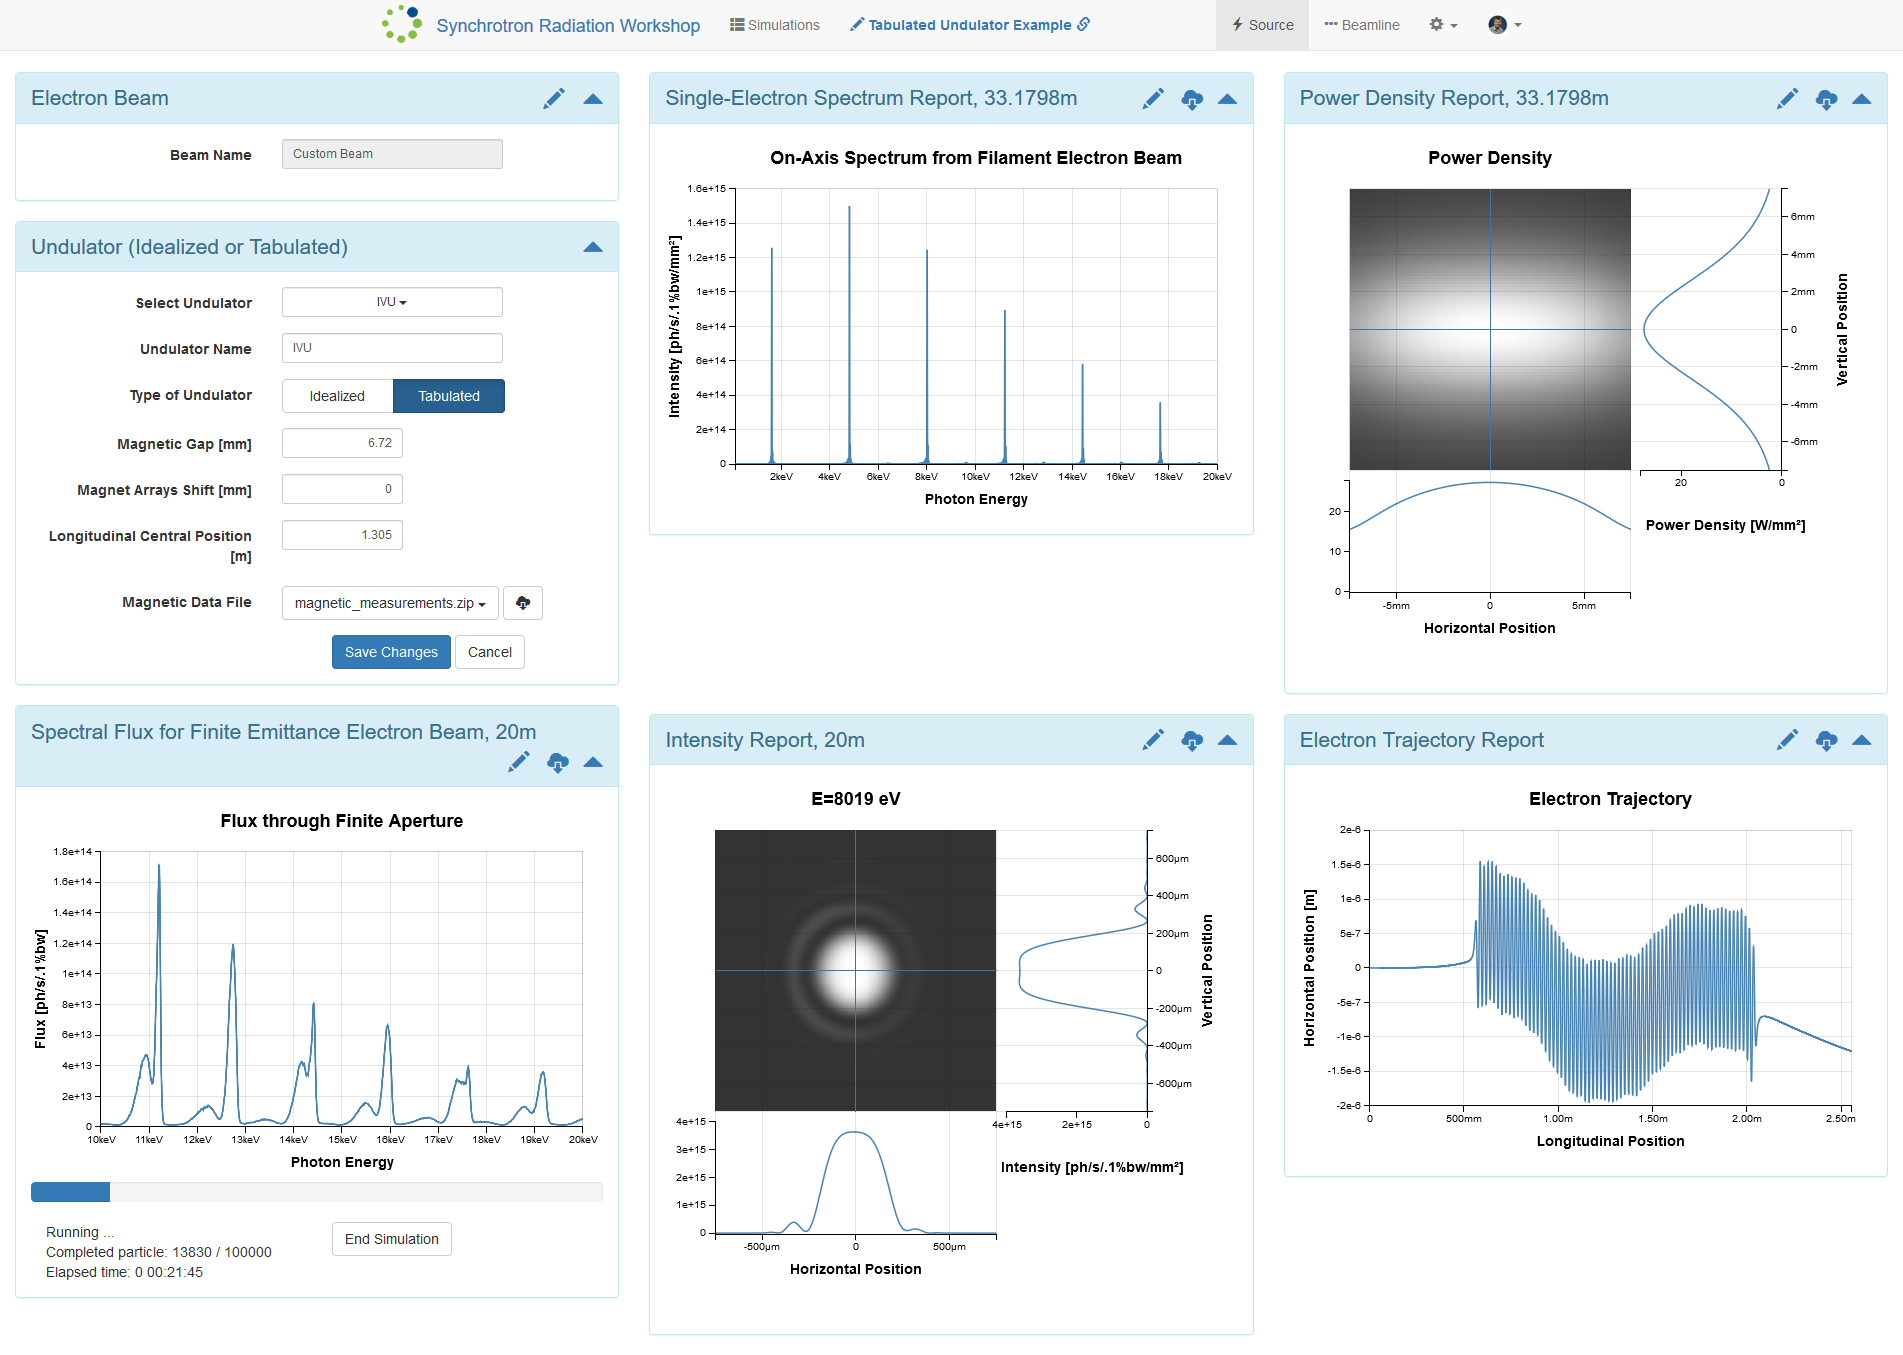
\includegraphics[width=0.95\linewidth]{images/source_page.png}
\end{figure}

\end{block} 

\begin{block}{\faSignOut{} \faEllipsisH{} \faBullseye{} Beamline page}
\vspace{-1.0cm}

\begin{figure}
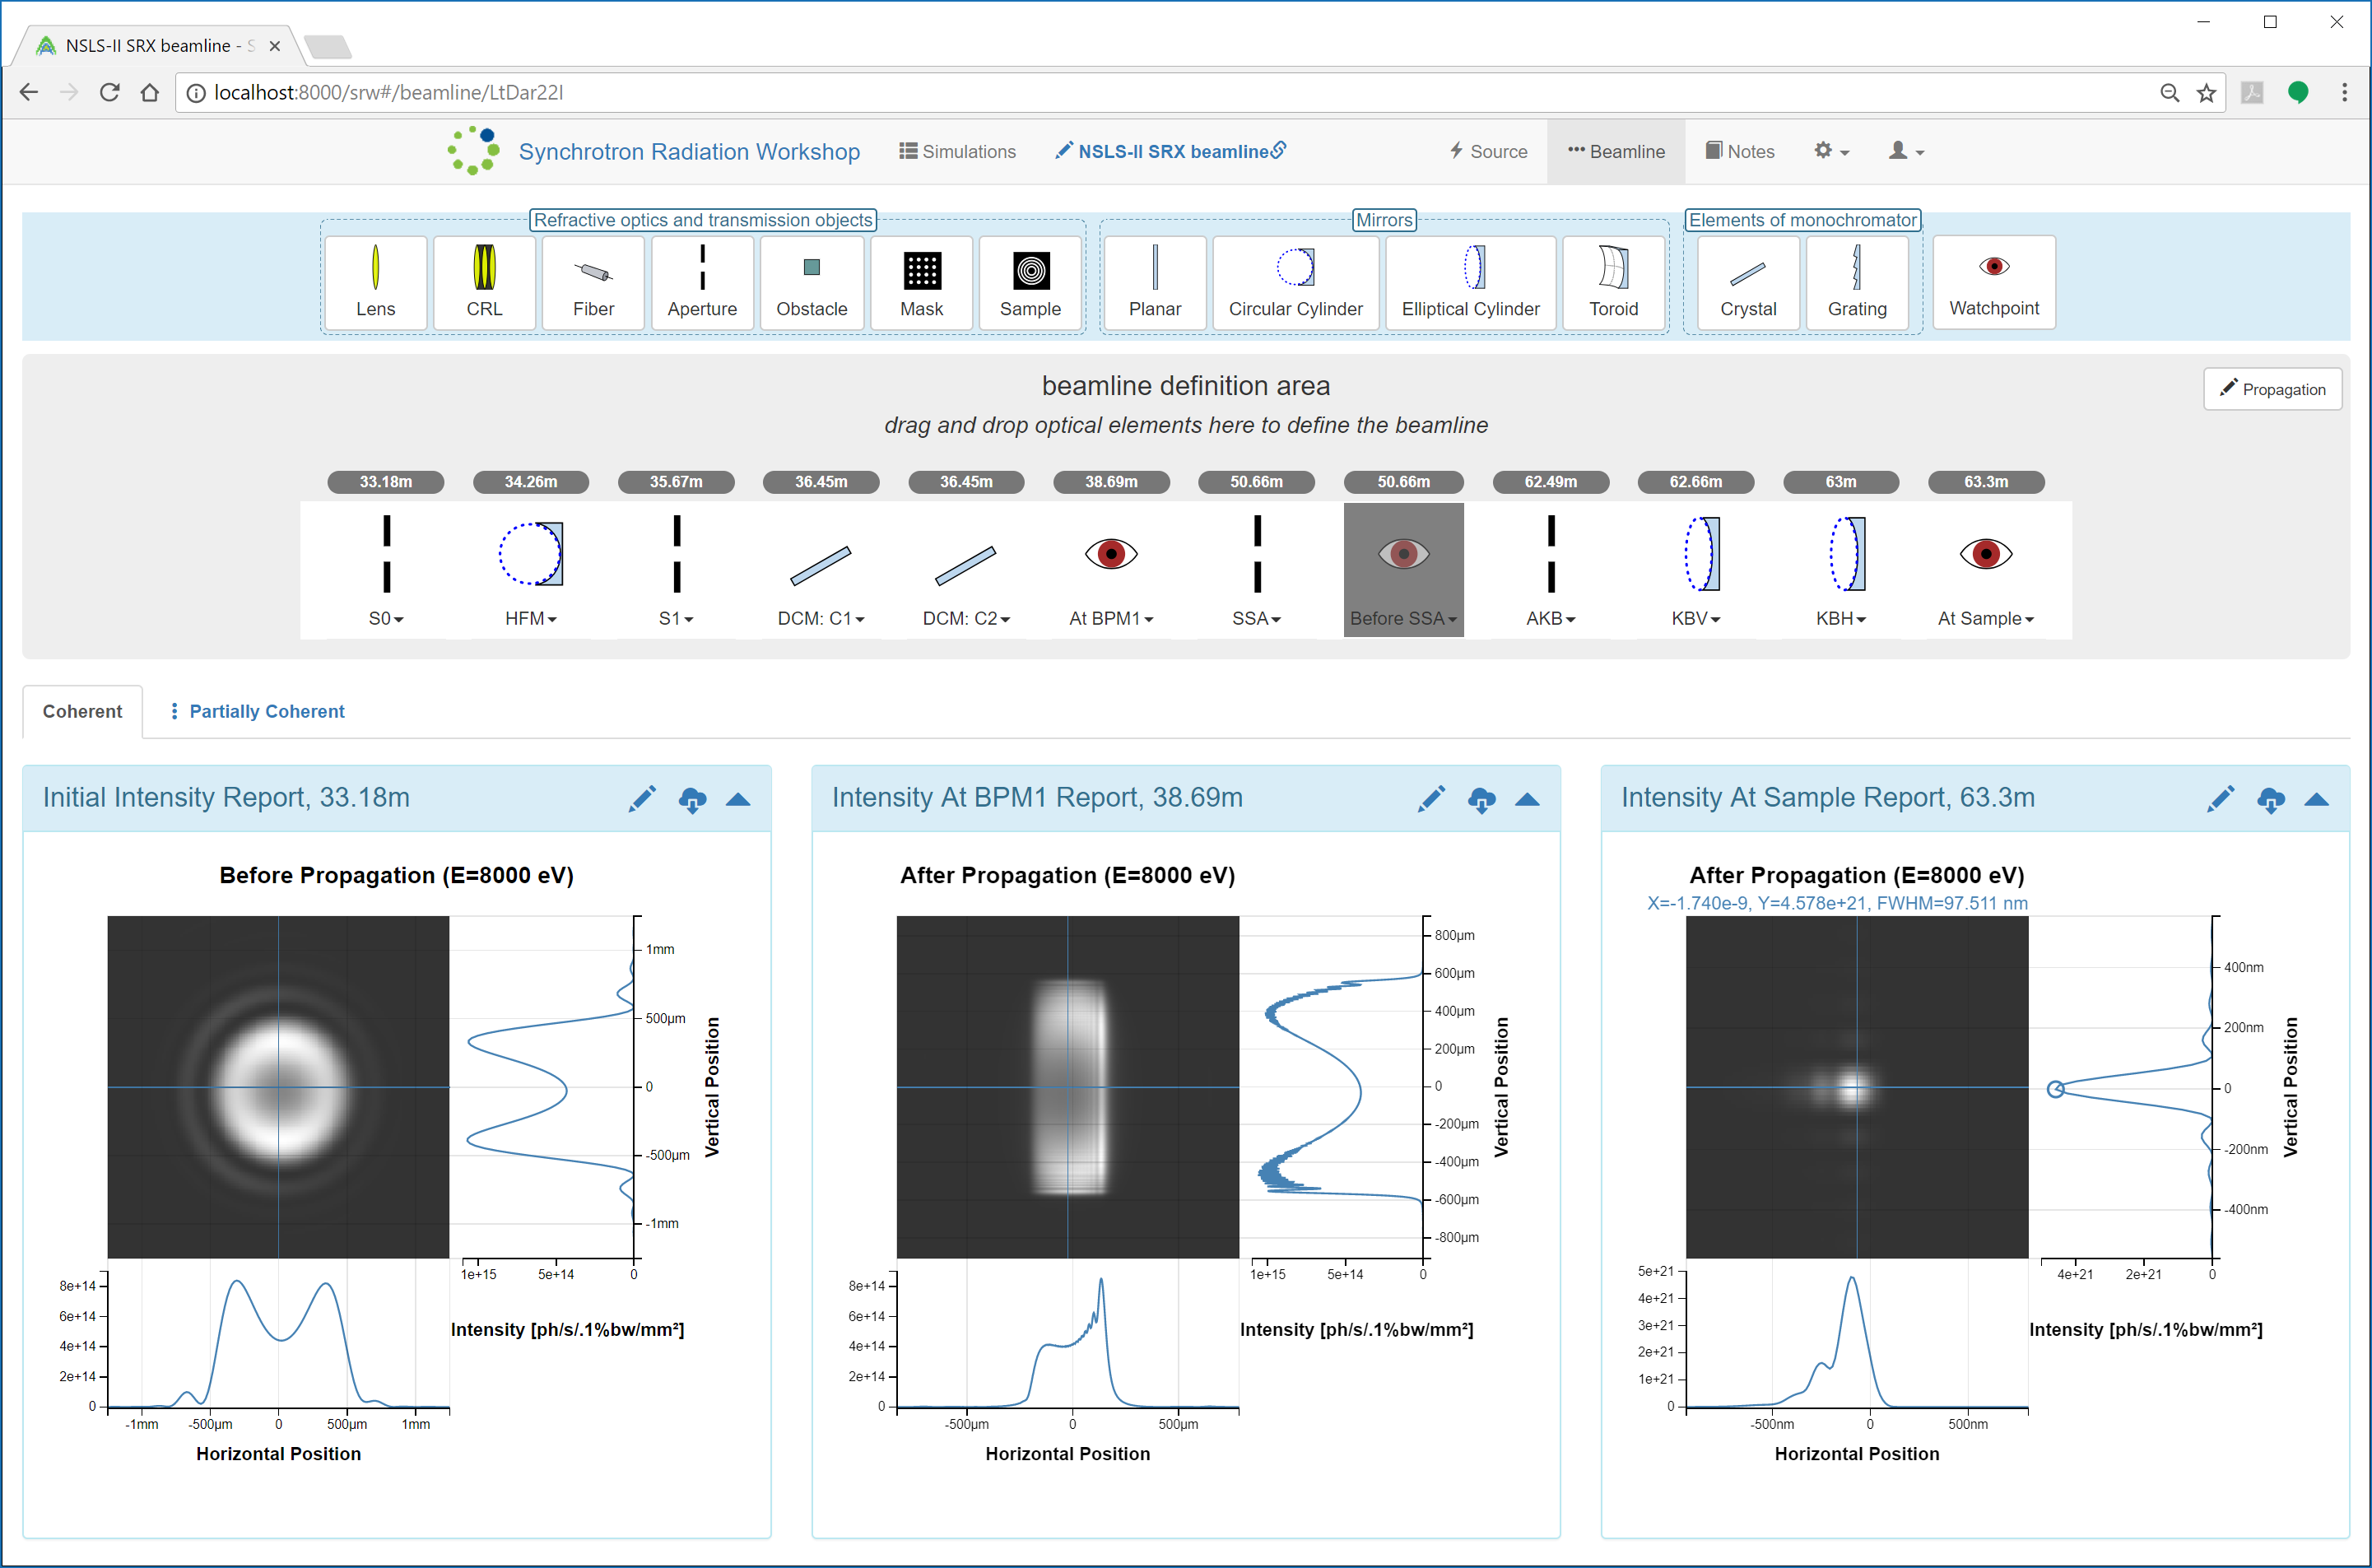
\includegraphics[width=0.95\linewidth]{images/beamline_page.png}
\end{figure}

\end{block}


\begin{block}{\faSpinner{} Comparison of SRW and SHADOW3 simulations}

\begin{figure}
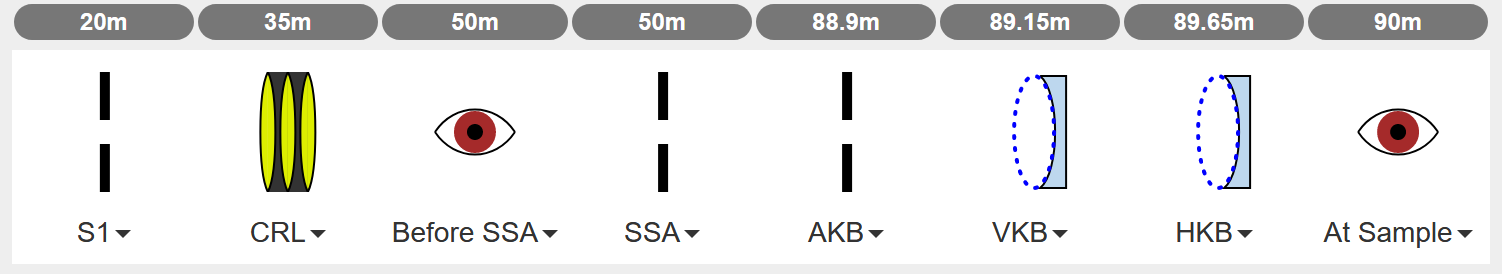
\includegraphics[width=0.6\linewidth]{images/imaginary_beamline.png} \\
\vspace{1cm}
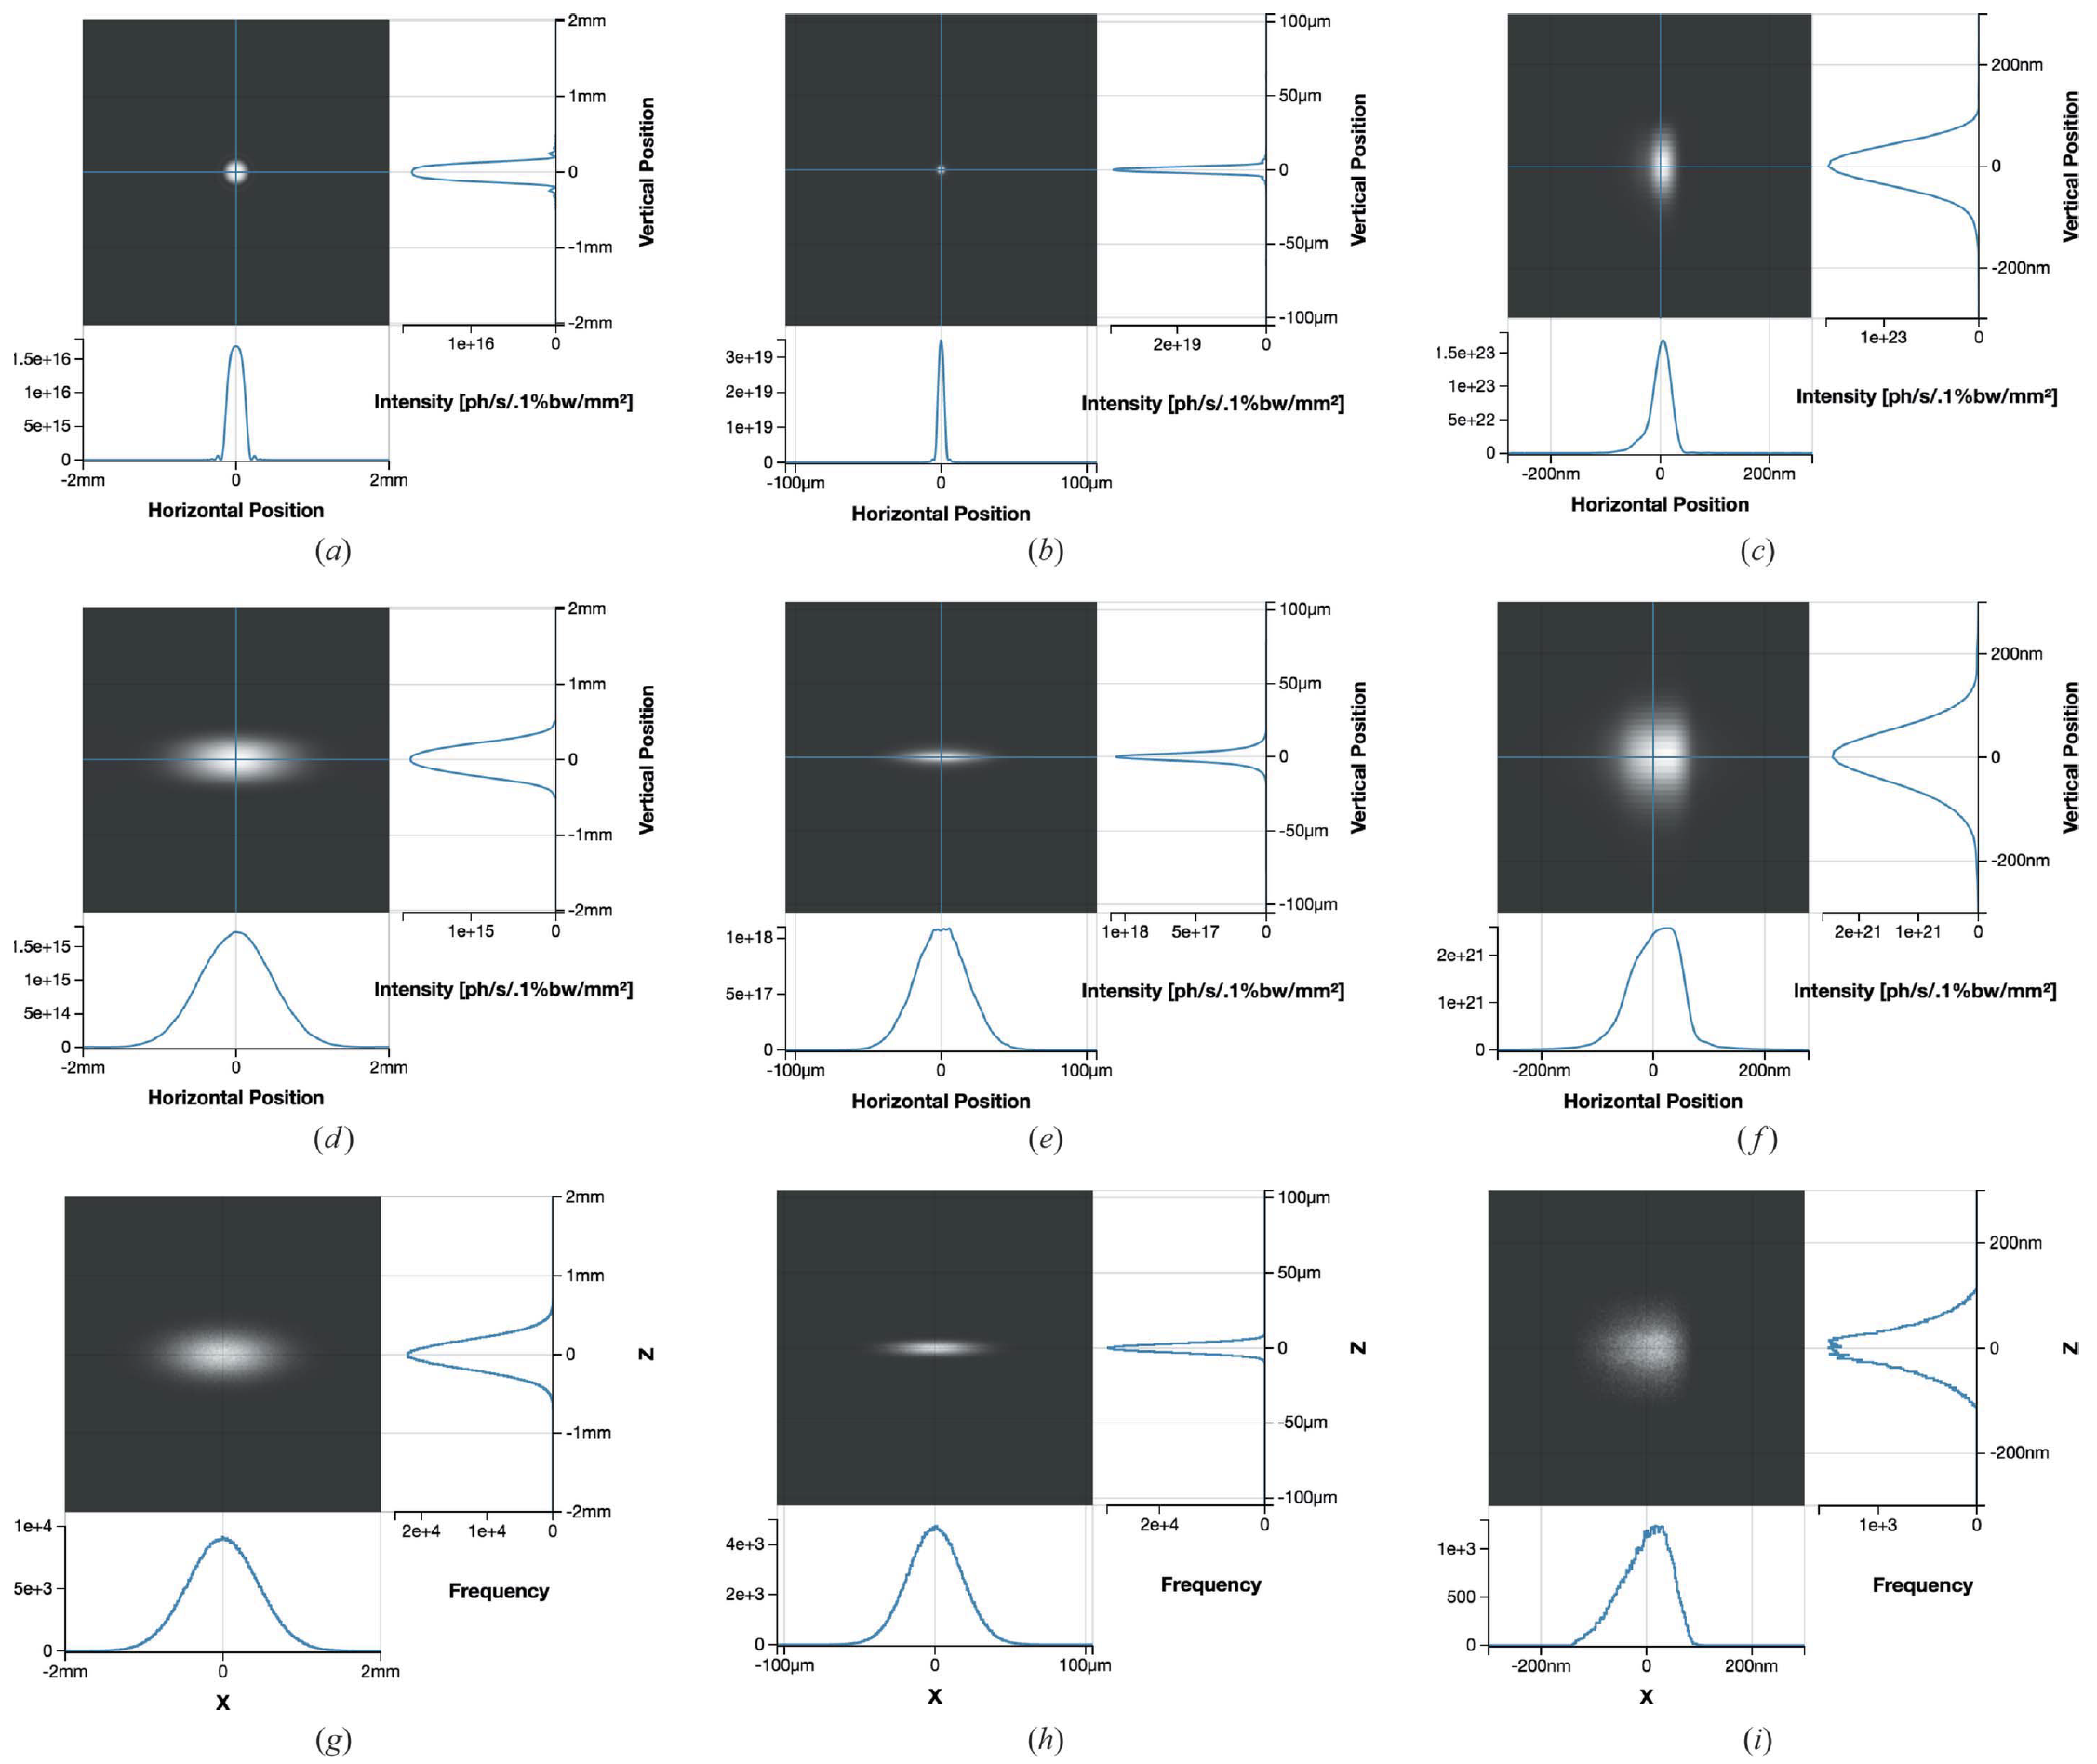
\includegraphics[width=0.8\linewidth]{images/srw-shadow_comparison.png}
\caption{Initial intensity report (at 20~m) and intensity reports for the
watchpoints ``Before SSA'' (at 50~m) and ``At Sample'' (at 90~m) (left to right)
in Sirepo. The first row corresponds to the single-electron (fully coherent) SRW
simulation, the second --- the multi-electron (partially coherent) SRW
simulation, and the third --- the fully incoherent SHADOW3 simulation.}
\end{figure}

\vspace{-0.8cm}

\begin{center}
\mylink{https://sirepo.com/srw\#/beamline/LA5qG1J1}~~~~~~
\mylink{https://sirepo.com/shadow\#/beamline/wsGlwMqv}
\end{center}

\end{block}

\end{column} % End of the second column



%-------------------------------------------------------------------------------
% Right single column
%-------------------------------------------------------------------------------

\begin{column}{\sepwid}\end{column} % Empty spacer column
\begin{column}{\onecolwid} % The third column


\begin{block}{\faSpinner{} Simulation of X-ray scattering from experimental samples}

\begin{figure}
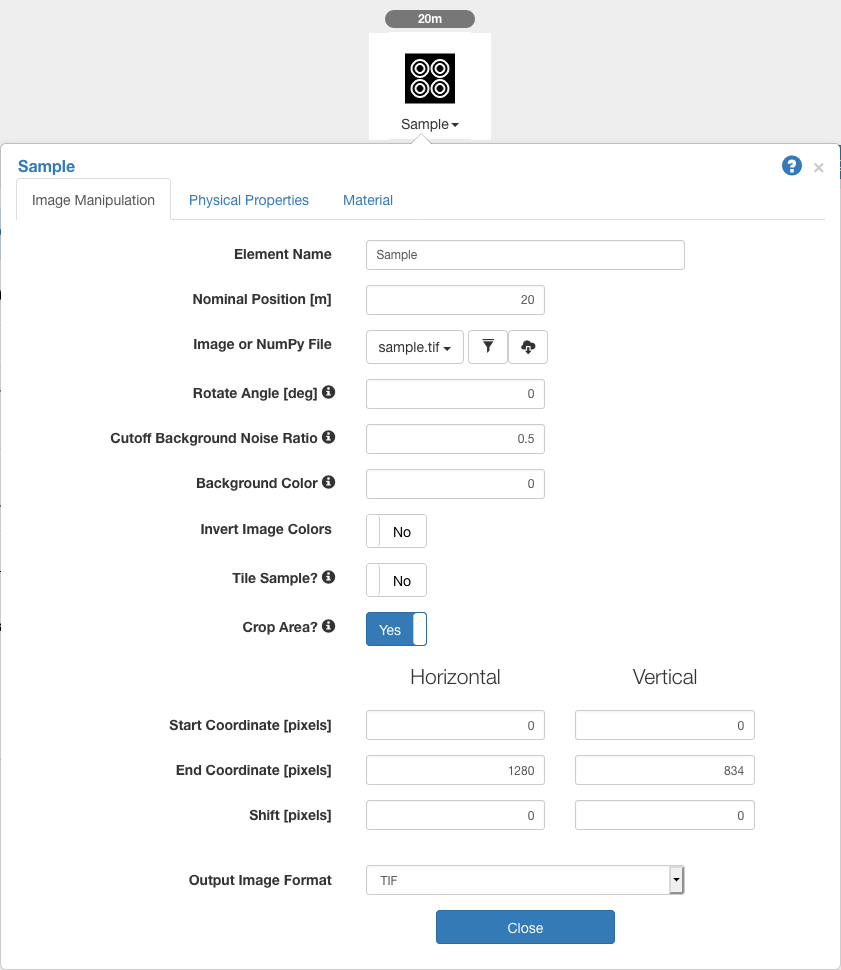
\includegraphics[width=0.9\linewidth]{images/sample_menu.png}
\end{figure}

\begin{figure}
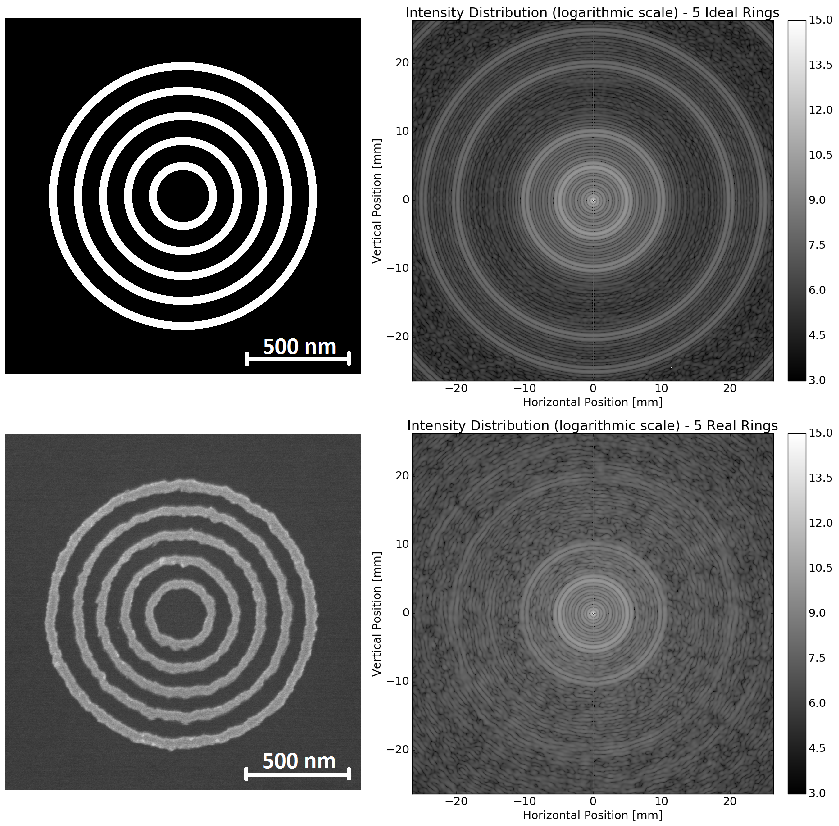
\includegraphics[width=0.8\linewidth]{images/samples_patterns.png}
\caption{Concentric rings sample (left) and simulated diffraction pattern 
created by it as observed at 4.81~m (right): `ideal' fabrication error-free case
(upper image plots) and the case of a sample object generated for simulations
from a real nano-fabricated sample (lower image plots). The outermost 
diameter/size of both samples is $\sim$1.35~$\upmu$m. The simulations were
performed with the NSLS-II CHX beamline layout.}
\end{figure}


The Sample optical element in Sirepo allows such simulations. Users can provide
an electron microscope image or a NumPy file describing a real or virtual
experimental sample, together with specified spatial resolution of the image and
thickness of the sample. The material of the sample can be specified in a
drop-down menu, and the refractive index decrement and attenuation length of the
material can be obtained automatically from the CXRO online database. Positions
of the sample can be specified relative to the source and the origin of the
incident beam frame.
\newline
\\
\textbf{Formats:}  image files (TIFF, PNG, JPEG, BMP, \ldots), or a NumPy array
file with the data of the sample image.
\newline
\\
Sample image $\rightarrow$ Python Image Library (PIL) $\rightarrow$ NumPy array
$\rightarrow$ crop ROI from the original image $\rightarrow$ SRW transmission
object (amplitude transmission and optical path difference calculations for each
pixel; the thickness of the material is proportional to the grey level of the
pixel) $\rightarrow$ wavefront propagation through the element and
drift space $\rightarrow$  diffraction pattern at the specified distance from
the sample.

\end{block}



%-------------------------------------------------------------------------------
%	ACKNOWLEDGEMENTS
%-------------------------------------------------------------------------------

%\setbeamercolor{block title}{fg=red,bg=white} % Change the block title color

\begin{block}{\faThumbsOUp{} Acknowledgements}

\small{\rmfamily{The authors are thankful for the financial support of this work
by the US DOE Office of Science, Office of Basic Energy Sciences under SBIR
awards DE-SC0006284 and DE-SC0011237.}} \\

\end{block}


%-------------------------------------------------------------------------------
%	REFERENCES
%-------------------------------------------------------------------------------

\begin{block}{\faBook{} References}
\nocite{*} % Insert publications even if they are not cited in the poster
\scriptsize{\bibliographystyle{unsrt}
\bibliography{sirepo} \vspace{-0.48cm}}

\end{block}


%-------------------------------------------------------------------------------
%	CONTACT INFORMATION
%-------------------------------------------------------------------------------

\setbeamercolor{block alerted title}{fg=black,bg=norange} % Change the alert block title colors
\setbeamercolor{block alerted body}{fg=black,bg=white} % Change the alert block body colors

\begin{alertblock}{\faSendO{} Contact Information}

~~~\faEnvelopeO~~\mylinkm{mrakitin@bnl.gov} \\
~~~\faGlobe~~\mylink{https://mrakitin.xyz} \\
~~~\faGithub~~\mylink{https://github.com/mrakitin} \\
~~~\faLinkedinSquare~~\mylink{https://www.linkedin.com/in/mrakitin} \\
~~~\faTwitter~~\mylink{https://twitter.com/mrakiti} \\
~~~\faPhoneSquare~~\mylinkt{+1~(631)~344--8299} \\

\end{alertblock}

%-------------------------------------------------------------------------------

\begin{minipage}[t]{0.25\linewidth}
\href{http://sirepo.com}{
\includegraphics[height=4.0cm]{images/qr_sirepo.png}}
\end{minipage}


\end{column} % End of the third column

\end{columns} % End of all the columns in the poster

\end{frame} % End of the enclosing frame

\end{document}
